\section{OLD STUFF: Implementation}
\label{sec:old-arch}

{\color{red} This section is relevant but needs major revisioning!}

% \begin{figure*}[!hbt]
% \centering
% 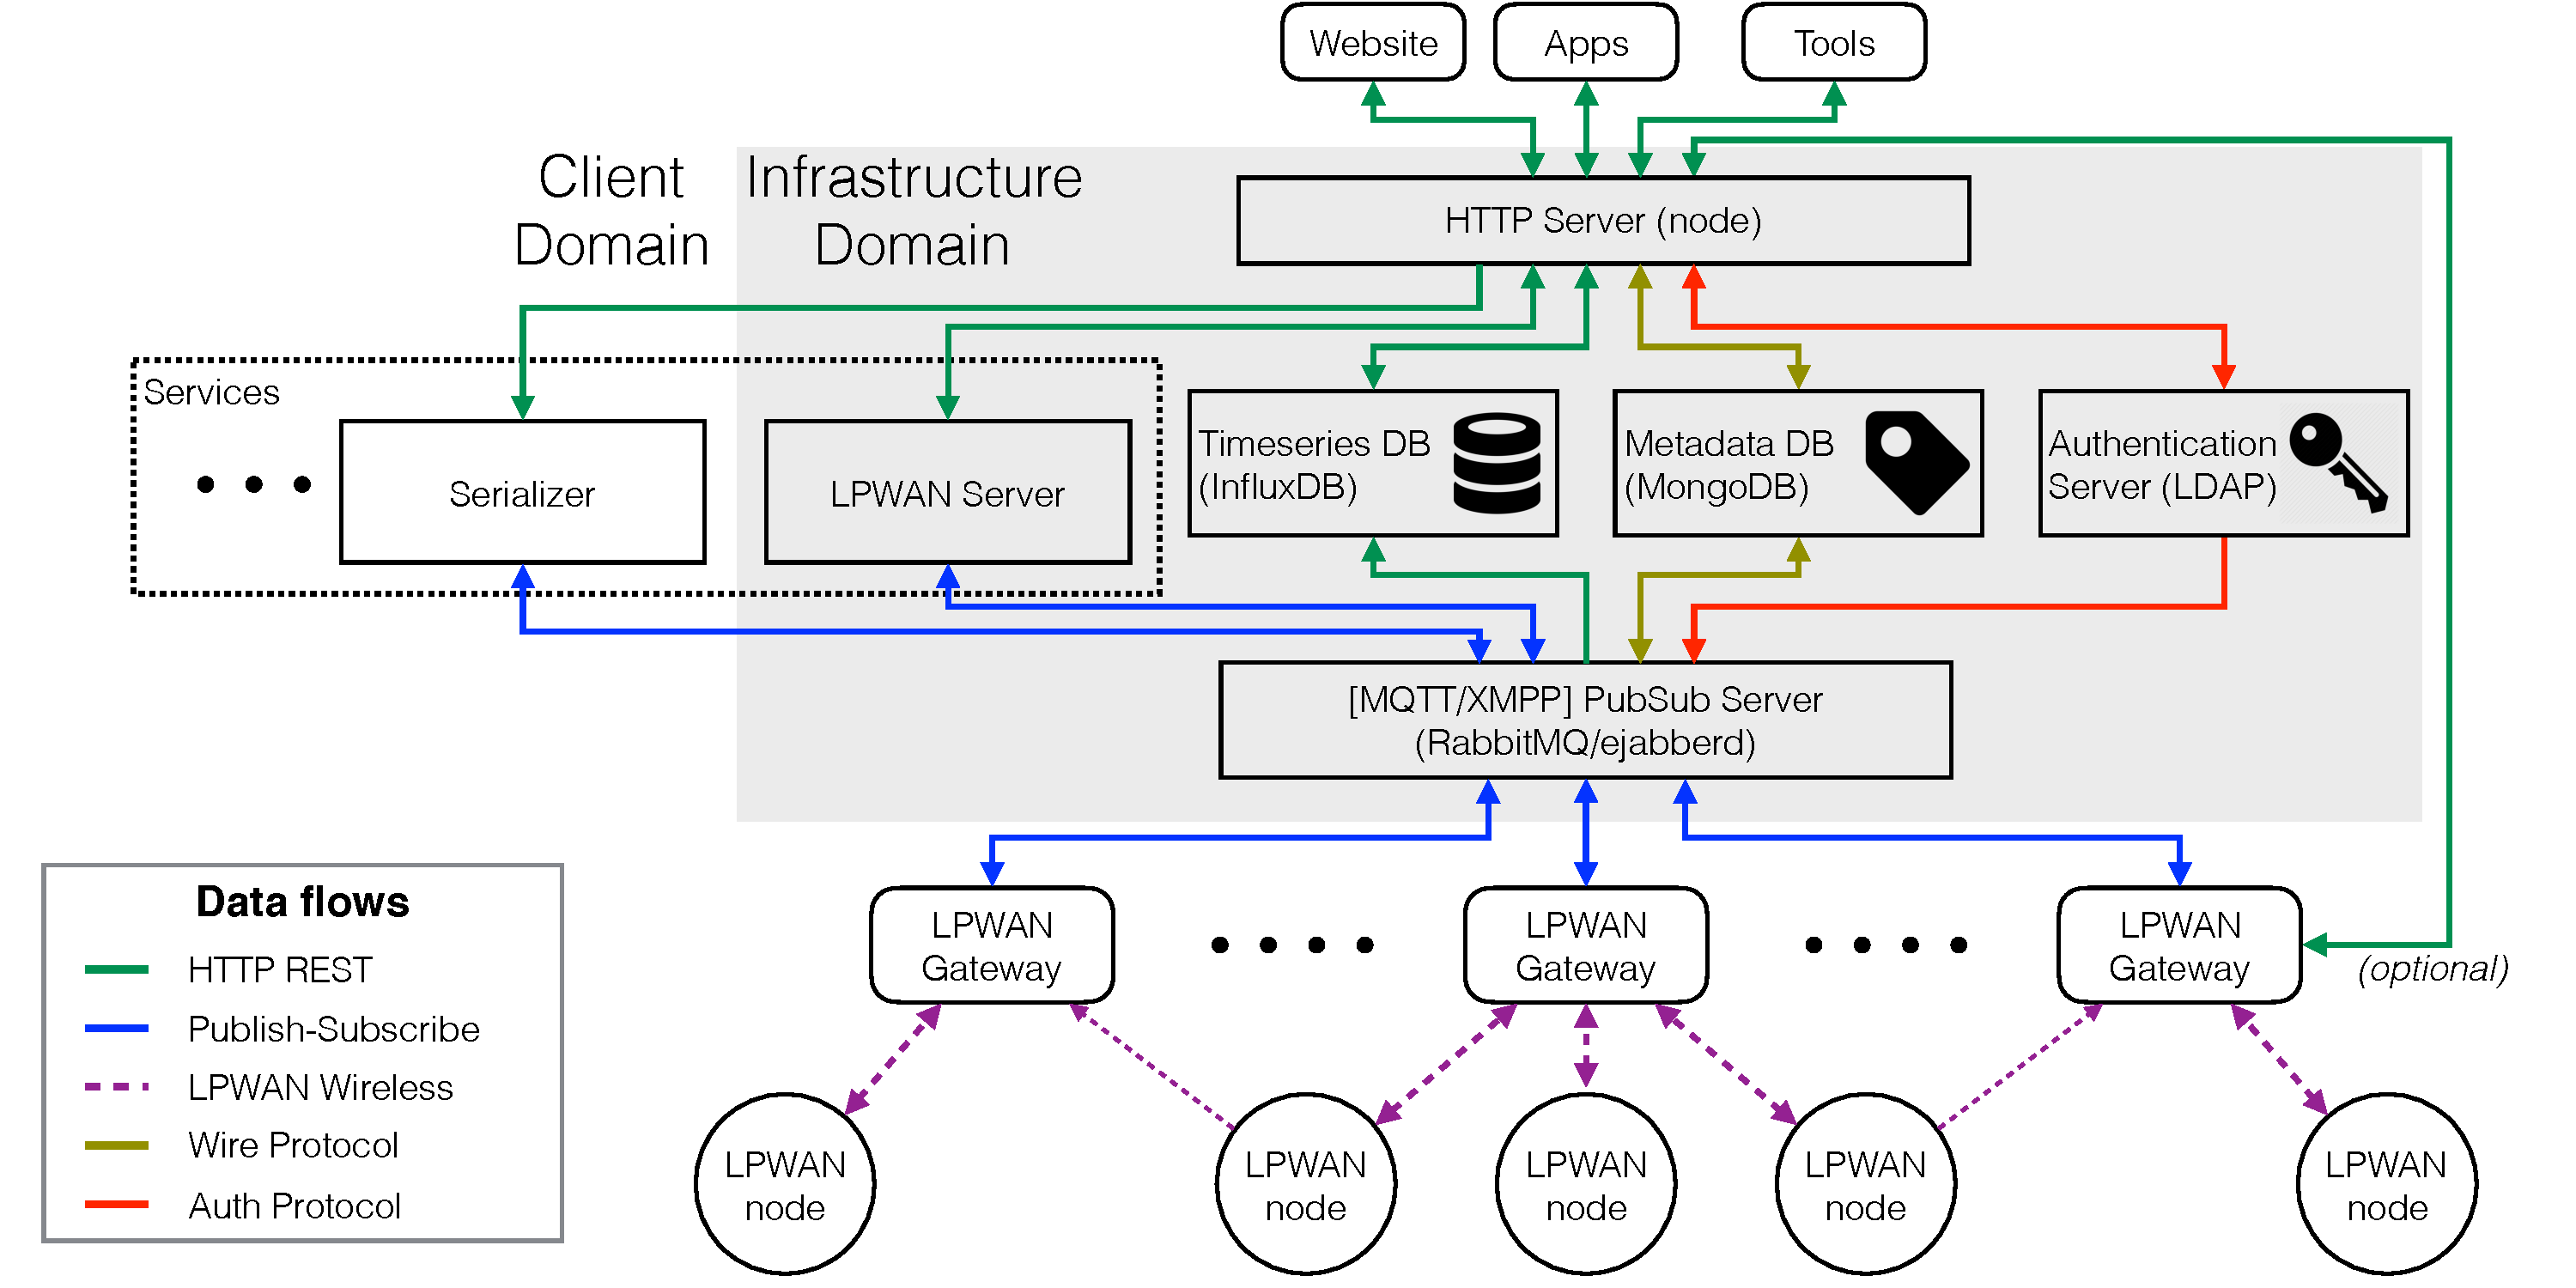
\includegraphics[width=0.6\textwidth]{figures/openChirp_architecture}
% \compactimg
% \caption{System Architecture}
% \label{fig:openchirp-arch}
% \end{figure*}


\begin{figure}%[!ht]
\centering
\compactimg
\subfloat{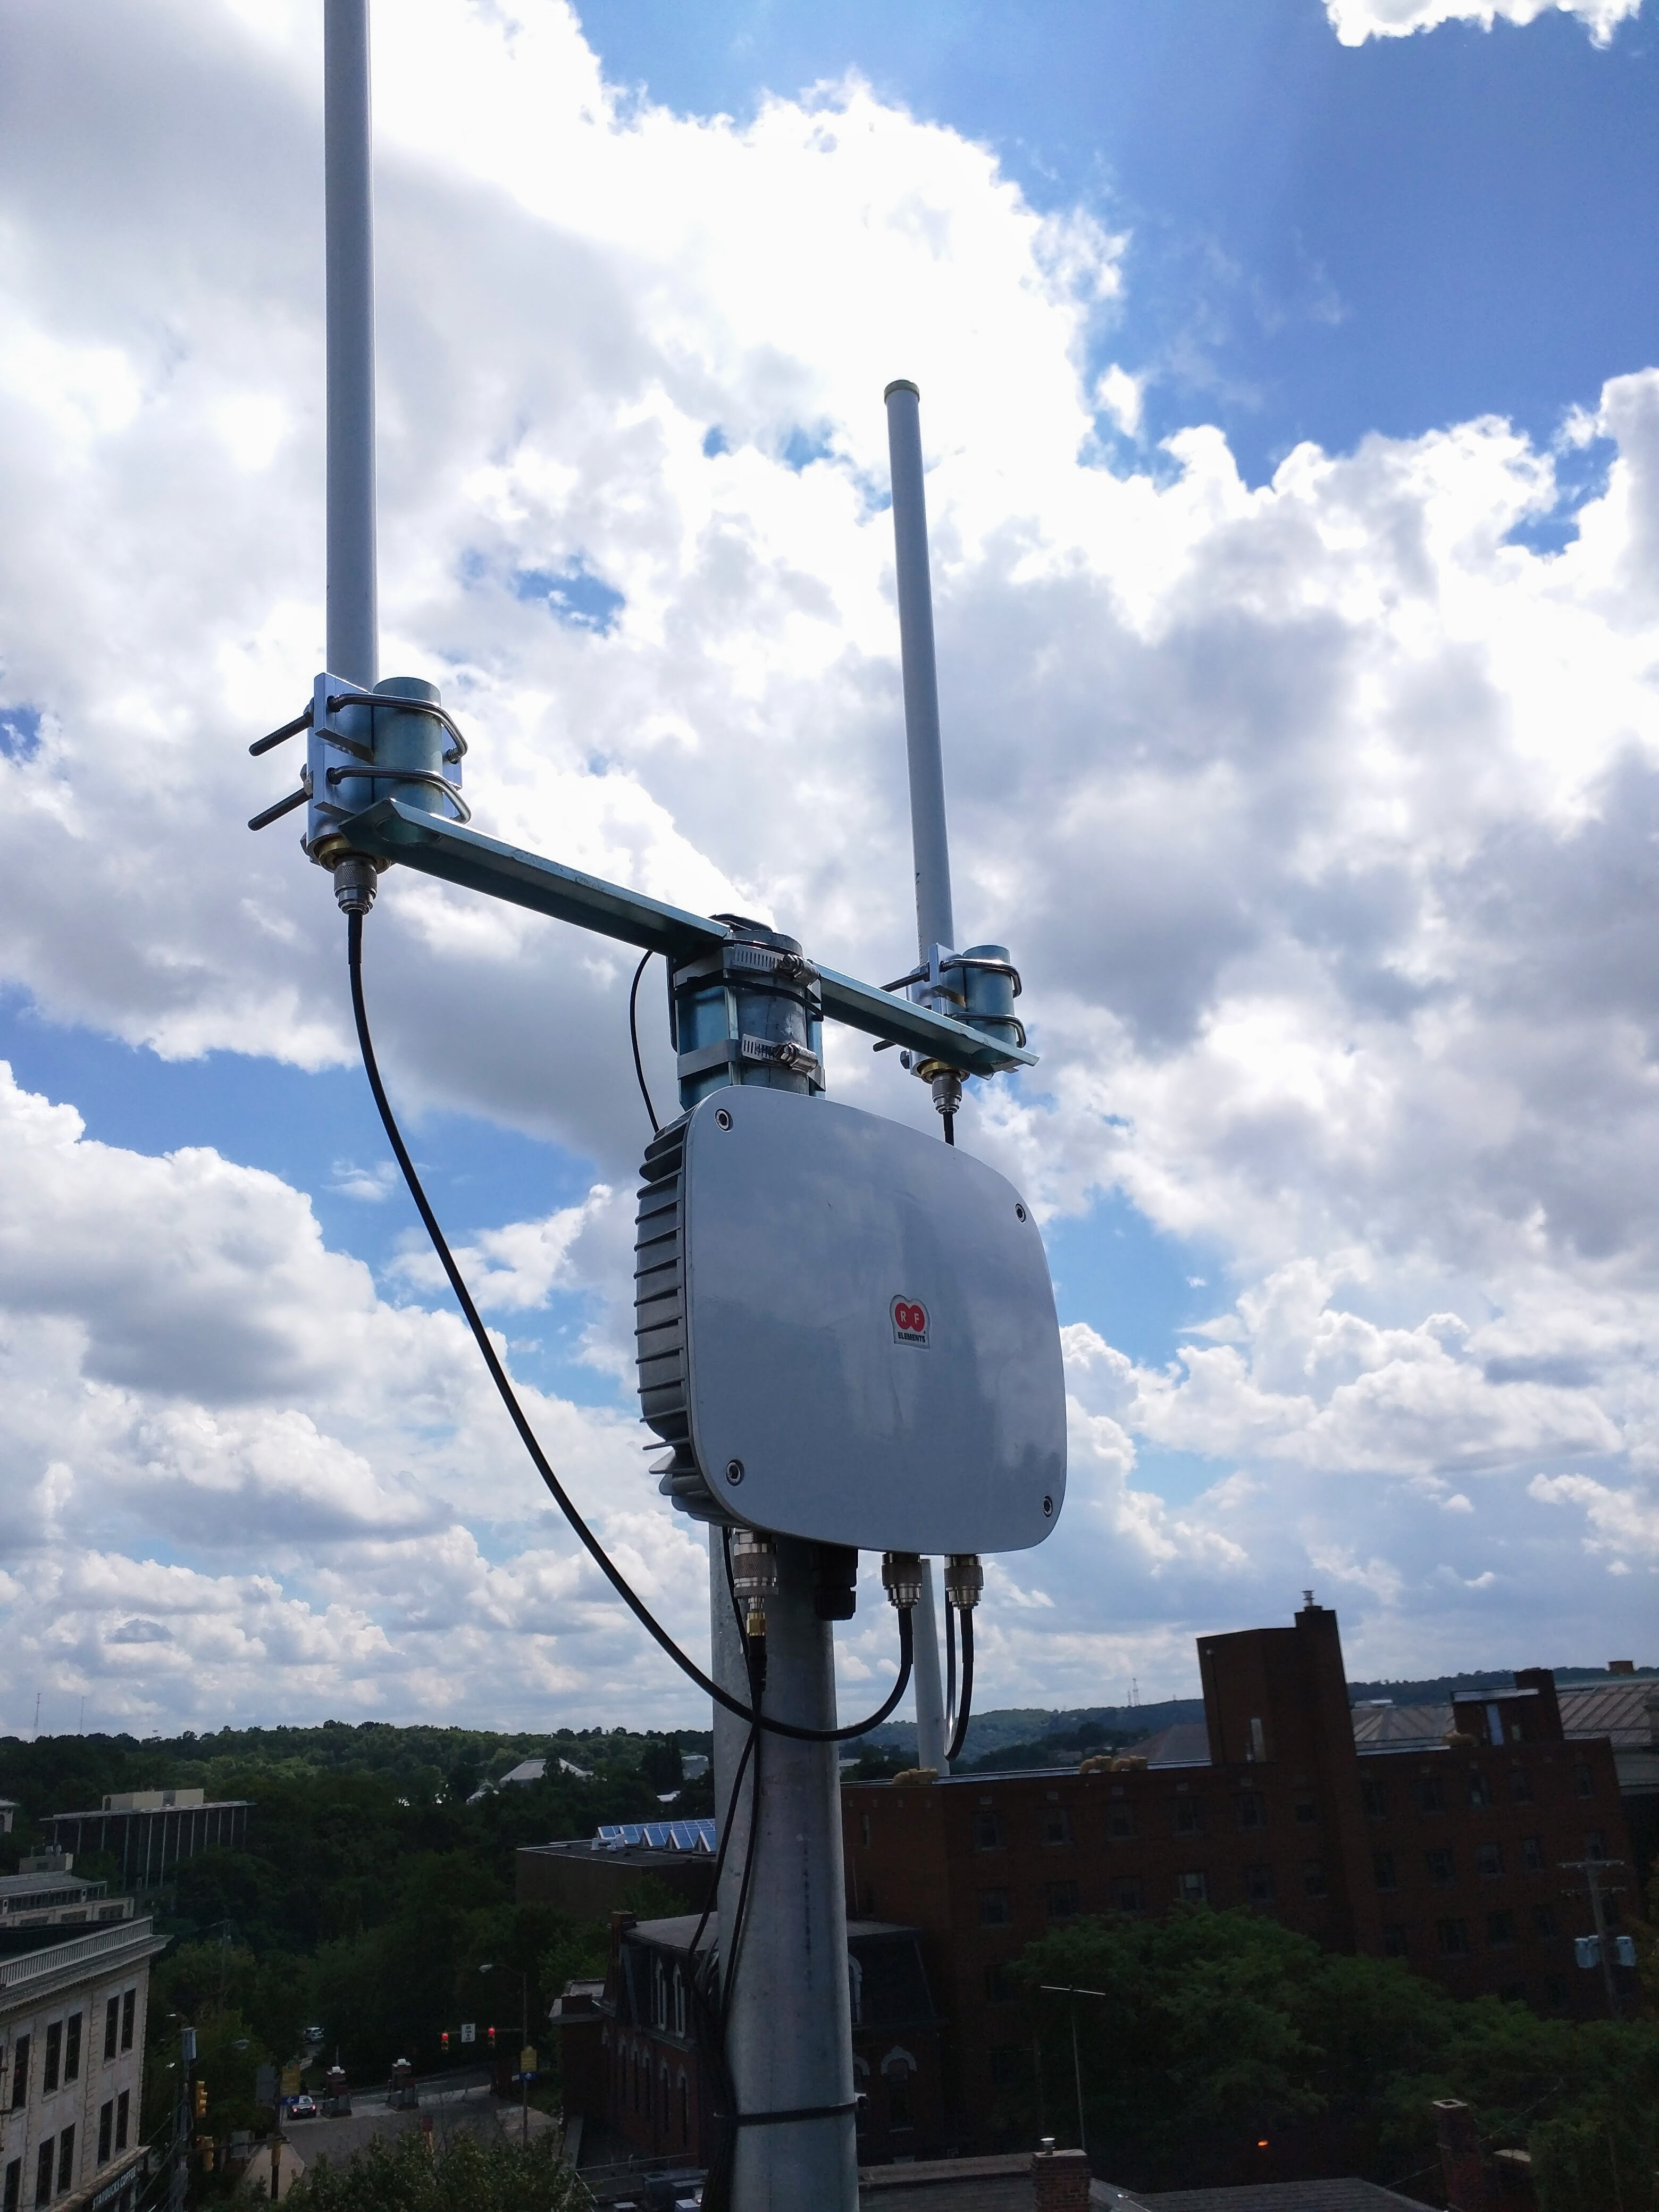
\includegraphics[height=3.9cm]{figures/gateway_deployment.jpeg}
\label{fig:gateway-photo}}
\hfill
\subfloat{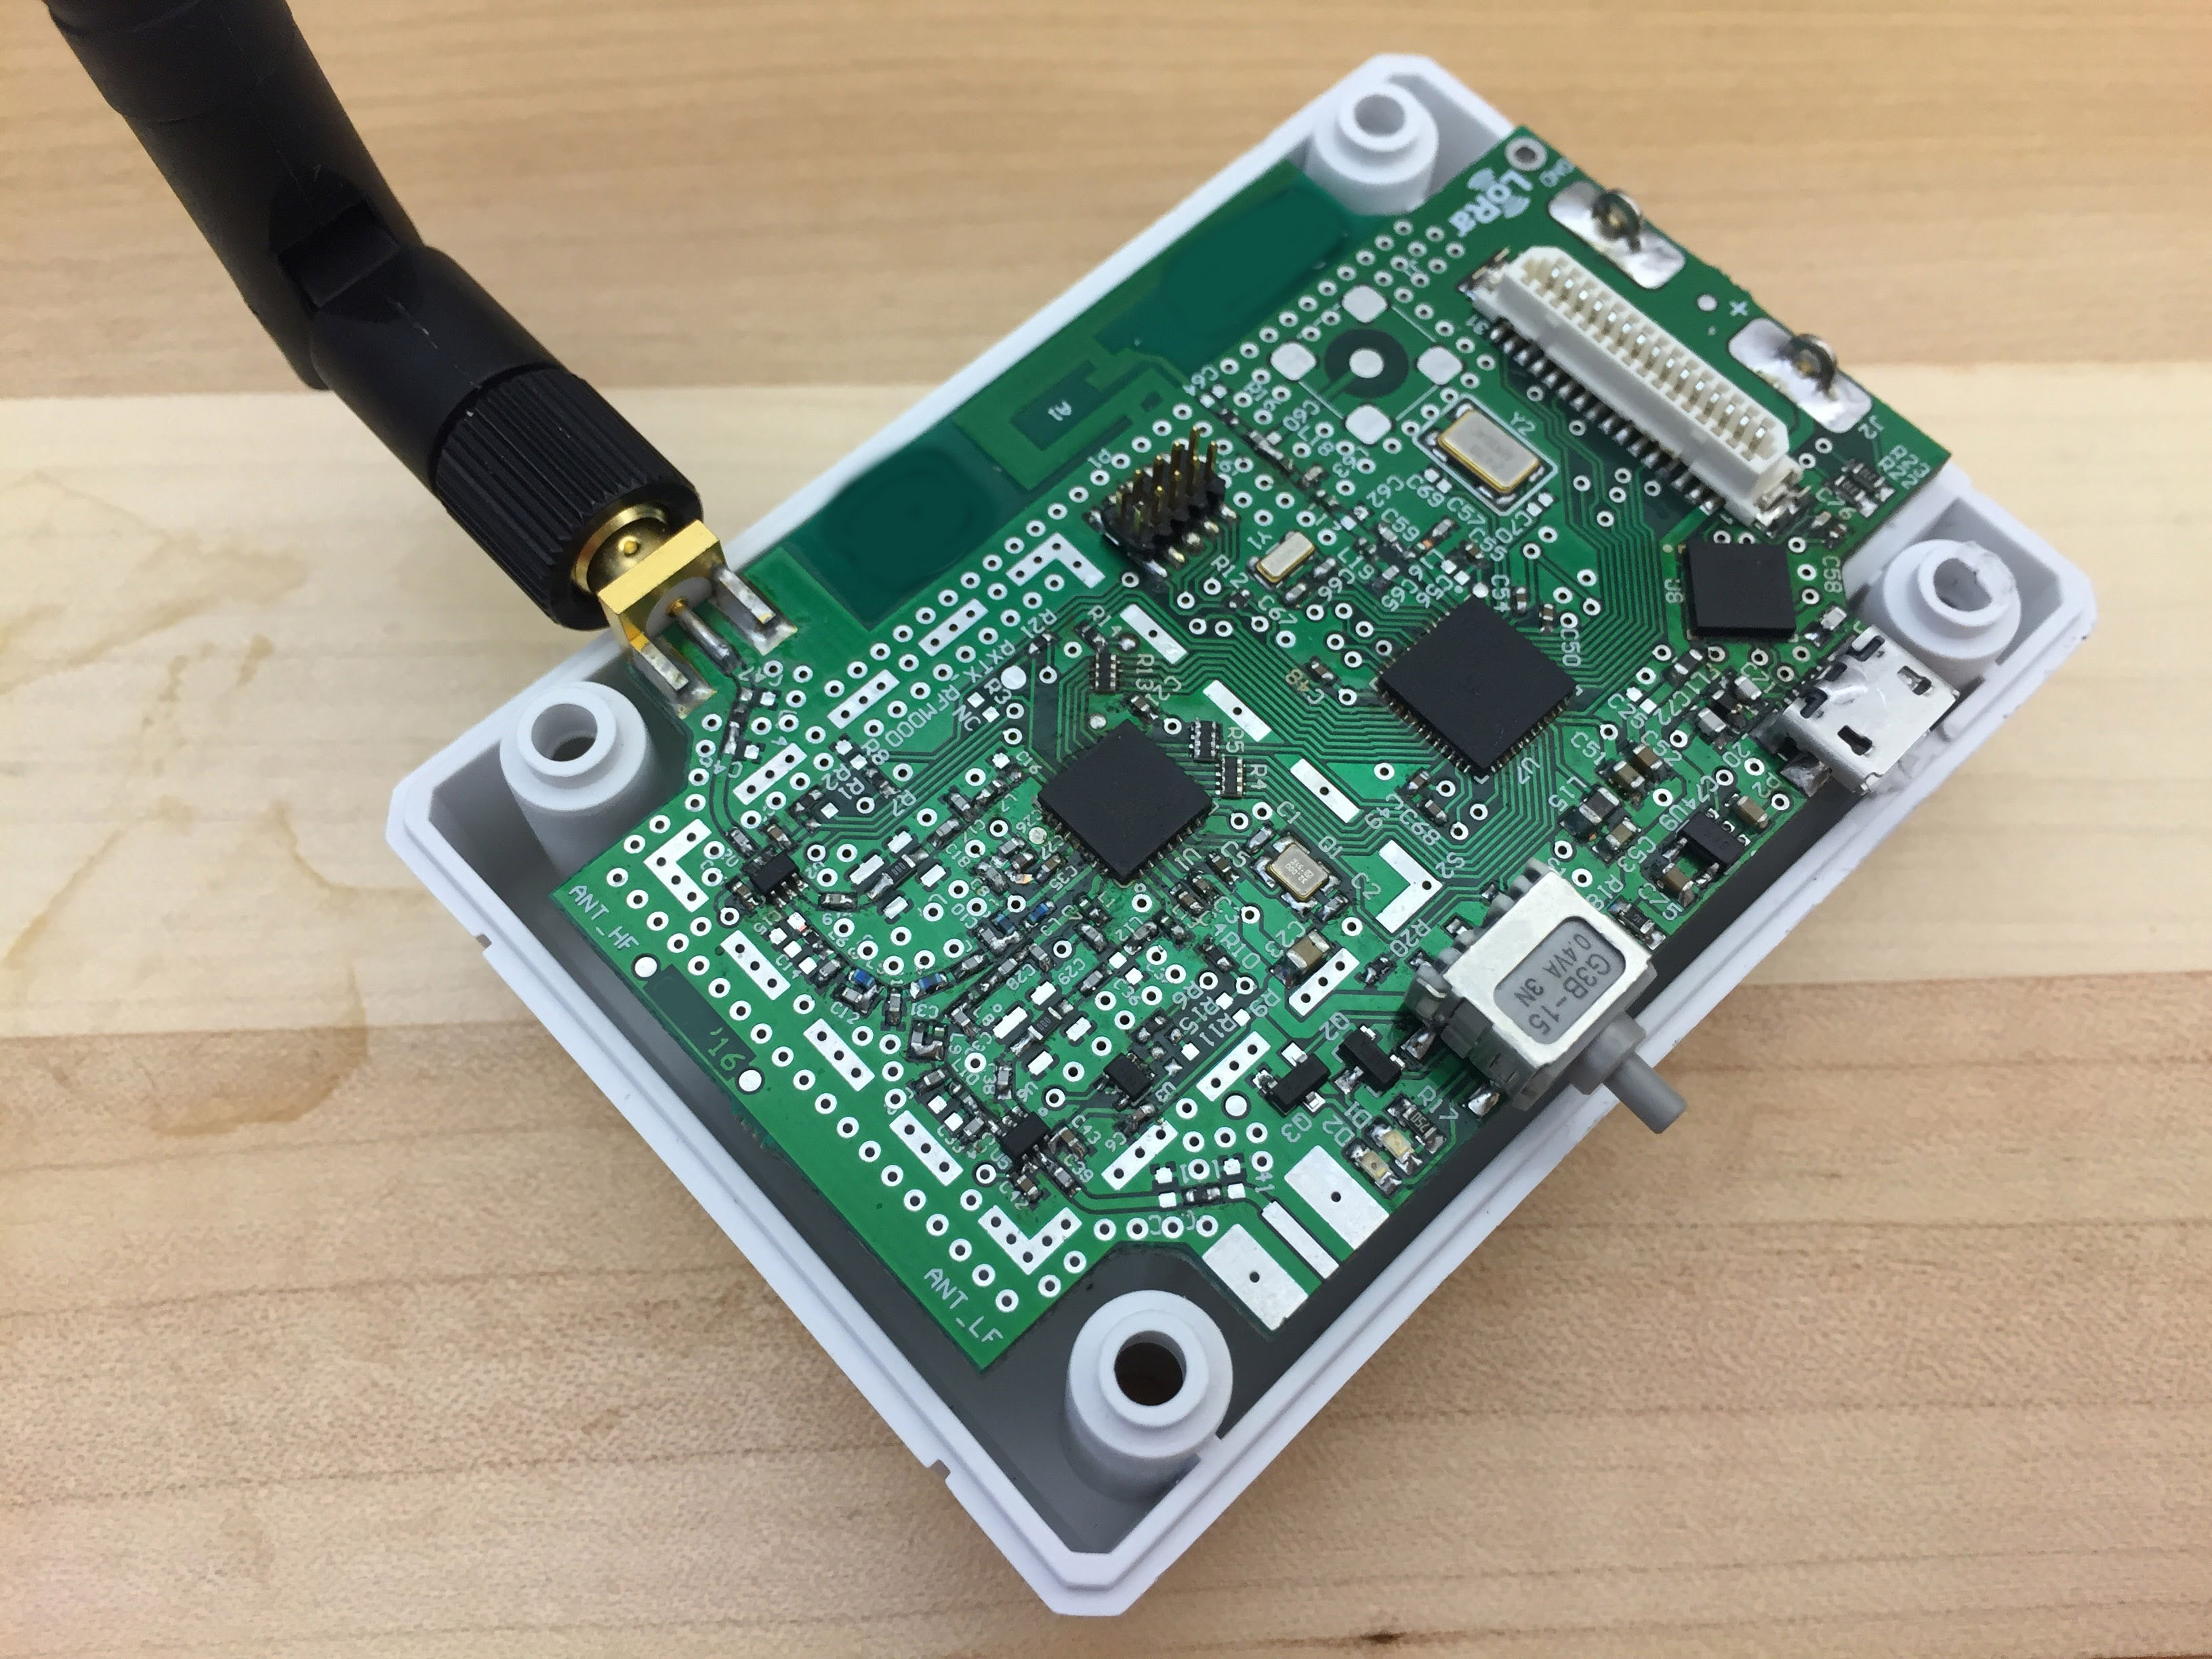
\includegraphics[height=3.9cm]{figures/receiver_anon.jpg}
\label{fig:lorabug-photo}}
\caption{Photo of our gateway (left) and a custom client node (right)}
\end{figure}



We implemented and evaluated our system extensively both through proof-of-concept experiments and trace-driven simulations to evaluate performance at scale. Our simulations were performed using traces gathered through a university campus-scale deployment of LoRaWAN base stations. We describe our hardware, testbed, measurements gathered, simulations and experiments below. 

%In the purest sense, a LoRaWAN server is responsible for delivering binary data blobs to and from an application.  To meet the needs of future multi-tenant city-scale sensing applications, we designed the OpenChirp which builds on top of LoRaWAN by adding a user management framework, application interface and a set of core services for performing data serialization (converting over-the-air binary data into a typed form with a schema), meta-data management and time series data storage.  

\vspace*{0.1cm}\noindent \textbf{Infrastructure Software Architecture: } {\color{blue} Add a description of the OC architecture. Refer to website for the problems it solves...}

\vspace*{0.1cm}\noindent \textbf{Base Station Hardware: } Our pilot deployment gateways used a standard single concentrator chipset that is able to receive on 8-channels simultaneously. Though ideal for low-cost deployments like what a user might deploy in their home, this does not exploit the entire LoRa spectrum.  For this purpose, we developed a more capable second-generation gateway, shown in \figref{64-chan-gw} that is able to operate on all 64-channels simultaneously. 
Similar to the 8-channel gateway, the 64 channel gateway is controlled by a single Raspberry Pi 3. Eight LoRa concentrator cards are used to interact simultaneously with 64 125kHz and 8 500kHz uplink (receive) channels and 8 500kHz downlink (transmit) channels. This spans the complete US LoRaWAN specified channel list from 902.3 to 914.9MHz for uplink and 923.3 to 927.5MHz for downlink. The radio cards are stacked in rows of four to optimize space inside the gateway enclosure. A Ublox GPS timing module is onboard to supply precise timestamps for incoming packets, synchronize time slots in LoRaWAN Class B, and to localize the gateways in the network. For future research, the board-to-board interface facilitates board stacks past that of dual 4 radio boards, while maintaining only a single USB connection to the Raspberry Pi host. This allows the radio board stack to be used with more powerful or generic machines that may not have GPIO and SPI peripherals. Additionally, the radio cards are secured into PCI Express Mini connector that expose many common wire protocols, which ensures upgradeability. We include an RTL software-defined radio for sensing of white spaces and listen-before-talk (LBT) functionality. For extended use in rough outdoor environments, we hardened the deployed hardware (weather-resistant design) and software (watchdog resets). The gateway is fully network connected and power using Power-Over-Ethernet(POE). \figref{gateway-photo} shows one of our four pilot rooftop gateways.


% \begin{figure}%[!htb]
% \centering
% 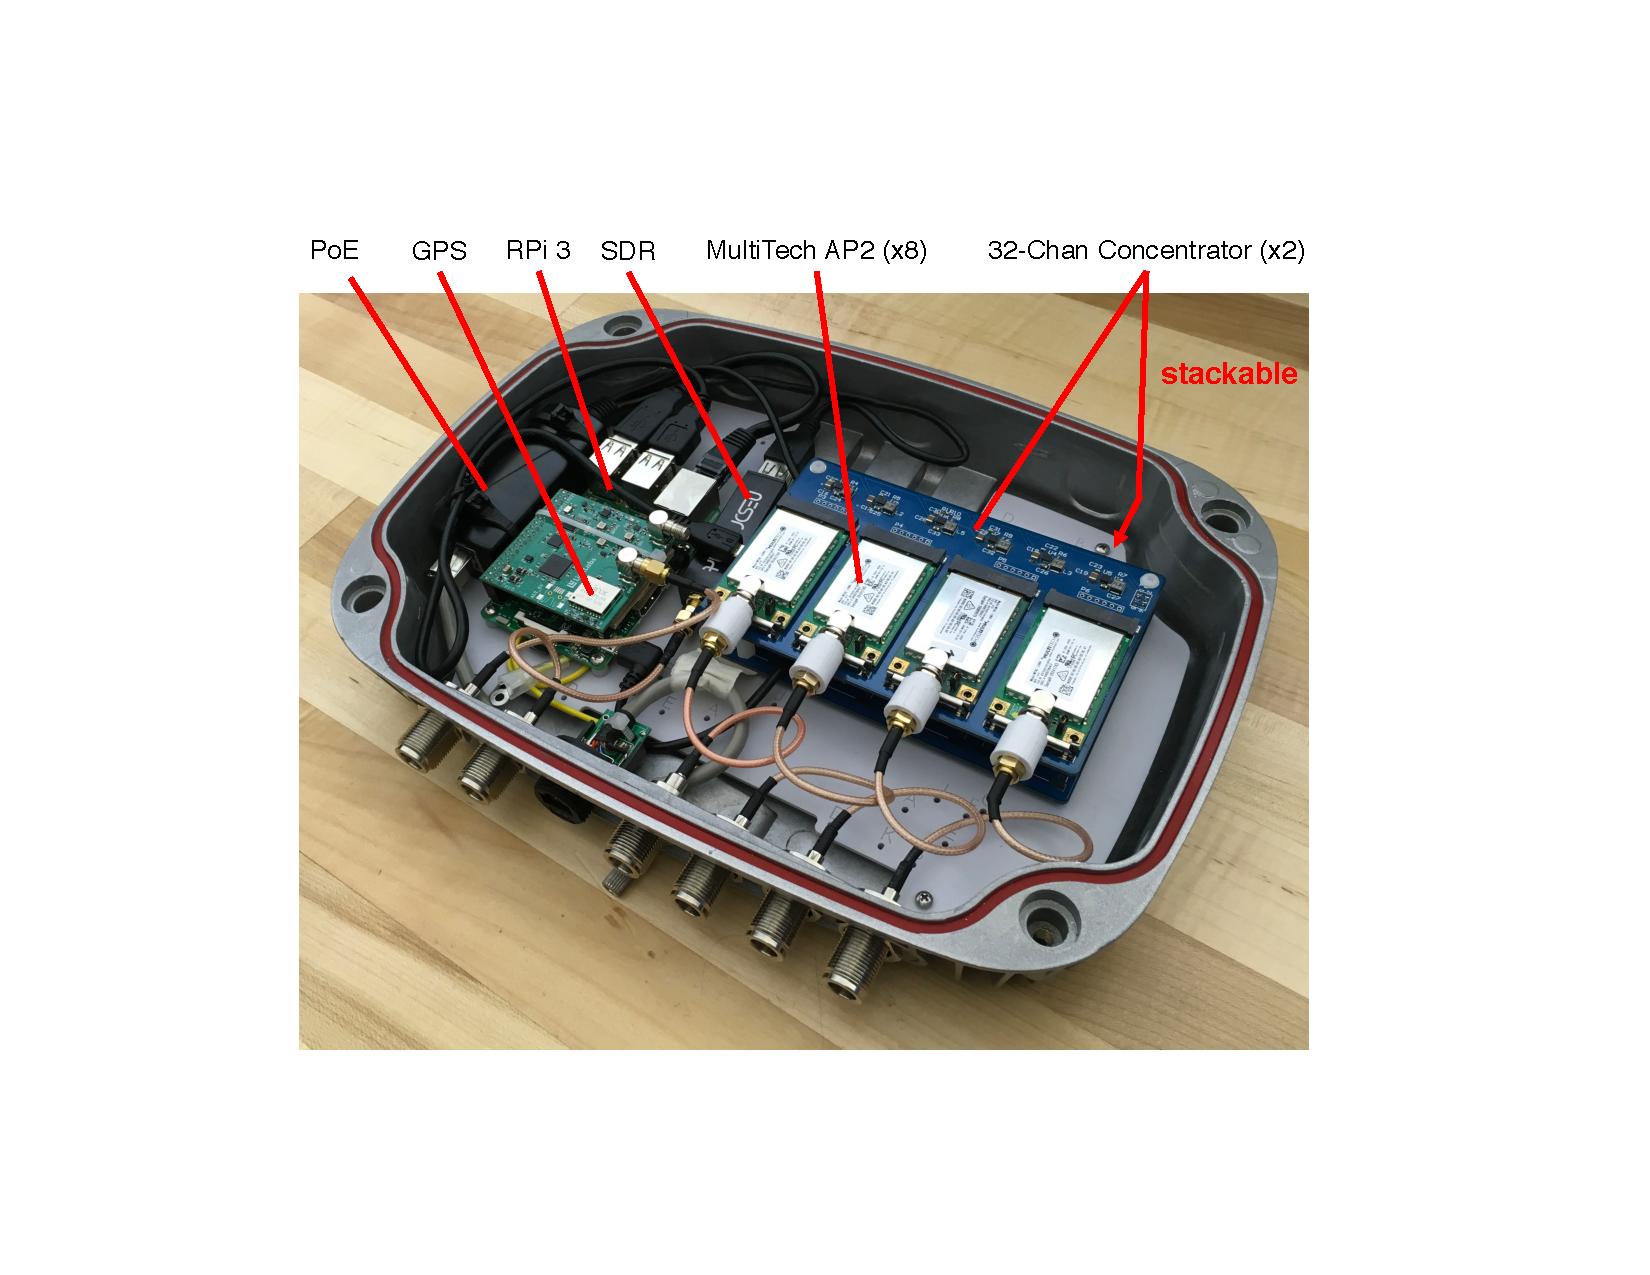
\includegraphics[width=0.4\textwidth]{figures/64-chan-photo.pdf}
% \compactimg
% \caption{Custom 64-channel gateway}
% \label{fig:64-chan-gw}
% \end{figure}

\begin{figure}%[!b]
\centering
%\compactimg
\compactimg
{\renewcommand{\arraystretch}{0}
\begin{tabular}{@{}c@{}}	
\subfloat{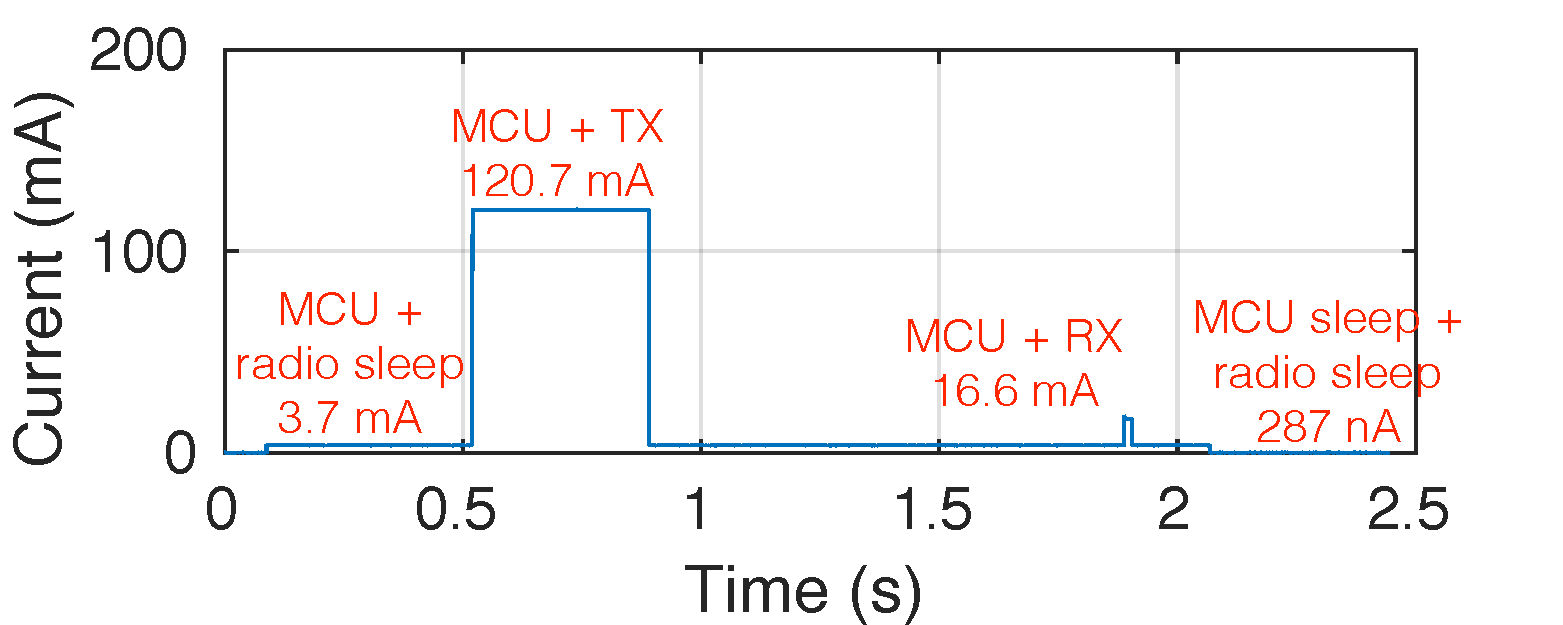
\includegraphics[width=0.4\textwidth]{figures/bug_power_trace_annotated} % NOTE: keep the \compactimg inside the subfloat comment to save space between the two images
\label{fig:power-trace}
} \\
\subfloat{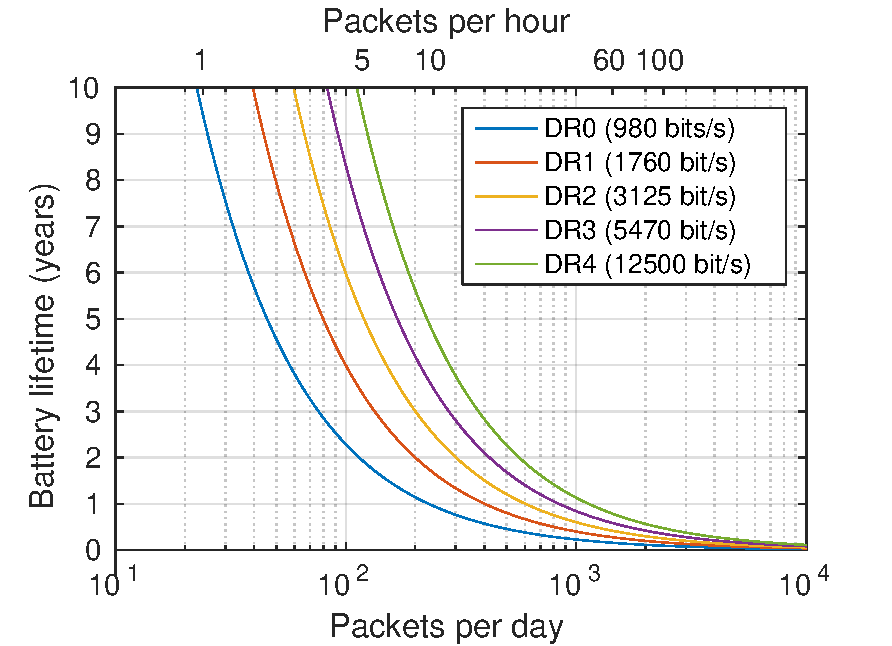
\includegraphics[width=0.4\textwidth]{figures/LoRaBug_AA_lifetime_semilog}
\label{fig:lifetime-estimates}
\compactimg}
\end{tabular}}
% \compactimg
\caption{(above) Custom LoRa client current consumption over time for transmitting a packet and then checking for an ACK from the gateway. (below) Lifetime of a custom LoRa client powered by two AA batteries at various operating points based on a measured energy profile.}
\end{figure}

{\color{red} Most of the custom client arguments like other platforms lacking BLE are not relevant anymore}

\vspace*{0.1cm}\noindent {\bf Custom LoRa Client:}   We found that many existing LoRa client implementations were not aggressively able to power down peripherals and few lacked BLE support which is extremely valuable for device provisioning. For this reason, we developed an open-source, low-cost, low-power, and extensible LPWAN end-node hardware platform shown in \figref{lorabug-photo}. The custom client is powered by a Texas Instruments CC2650 microcontroller (MCU) with integrated 2.4 GHz IEEE 802.15.4 and Bluetooth Low-Energy (BLE) radios. It communicates to LoRa networks through a Semtech SX1276 LoRa radio. The node can be augmented with expansion modules for a variety of applications (e.g. environmental sensing, GPS localization and actuation). In addition to typical sleep states, the MCU has an ultra low-power sensor co-processor for sensor sampling and data aggregation, and a cryptographic accelerator that enhances the performance of security functions and reduces code-size. The custom client hardware is housed in a small plastic enclosure that accommodates two AA batteries. 

%\begin{figure}[!htb]
%\centering
%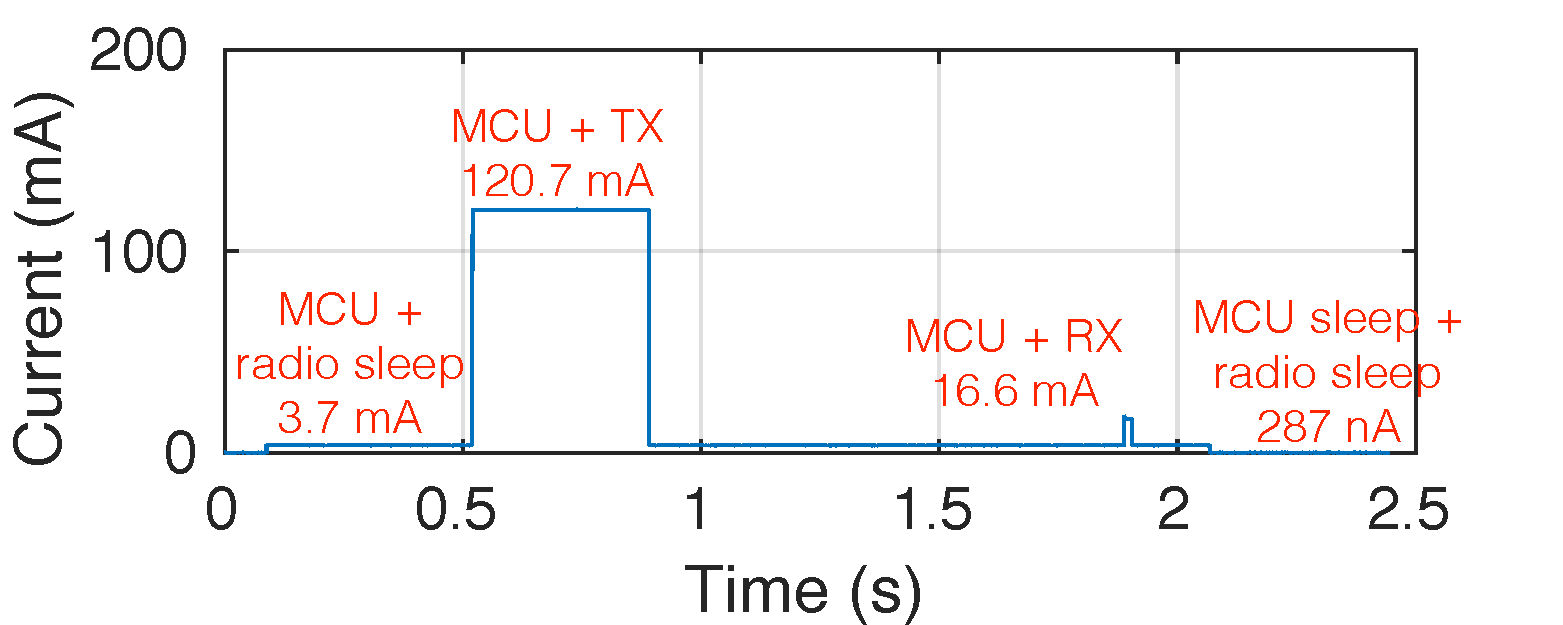
\includegraphics[width=0.4\textwidth]{figures/bug_power_trace_annotated.pdf}
%\compactimg
%\caption{{\color{blue} Add caption}}
%\label{fig:bug_power_trace}
%\end{figure}




Both our MCU and LoRa radio have multiple sleep and function states that consume varying amounts of power. In \figref{power-trace} we look at the current consumed by these devices while sending out 8 bytes of data and receiving an acknowledgment. The radio was configured for uplink communications with 125 kHz channel bandwidth, data rate of 980 bits/s, spreading factor of 10 and coding rate of $4/5$.  Based on a simple power model, we estimate the lifetime of these devices in \figref{lifetime-estimates} while operating on two 2000 mAH AA batteries (we make a conservative estimate of 60 \% usable energy and maximum shelf life of 10 years). Thus, with proper duty-cycling, the custom client can function and communicate for multiple years on simple batteries.





% \vspace*{0.1cm}\noindent{\bf Localization Testbed: } We conduct our localization experiments on a testbed composed of SX1276MB1LAS boards with an embedded LoRaWAN chip that
% is mBed compatible. We connect these boards with NUCLEO-L152RE boards with the mBed platform to program the LoRa chips to hop between a range of pre-specified frequencies. The boards operate at  center frequencies in the 433 MHz and 902 MHz ISM band over a bandwidth of 500~KHz or 125~KHz depending on the
% data rate the wireless channel supports~\cite{alliance2015lorawan}. We use the RTL-SDR~\cite{rtlsdr} platform to collect wireless channel measurements. The collected  wireless channels between transmitter-receiver pairs are aggregated at the base station, where they are processed using our C++/MATLAB based localization framework.









